\documentclass[twocolumn]{article}
\usepackage[spanish]{babel}
\usepackage[utf8]{inputenc}
\usepackage{graphicx}
\usepackage{booktabs}
\usepackage{amsmath}
\usepackage[margin=1in]{geometry}
\usepackage{url}

\title{Simulación de Sistema Coloidal Utilizando el Algoritmo de Verlet}
\author{Tu Nombre}
\date{Noviembre, 2024}

\begin{document}

\maketitle

\begin{abstract}
Este trabajo presenta un estudio detallado de la simulación de sistemas coloidales utilizando el algoritmo de Verlet con velocidades y el potencial de Lennard-Jones. Implementado en el lenguaje de programación Zig, nuestro modelo explora la dinámica de partículas coloidales bajo diversas condiciones iniciales. La simulación abarca cuatro escenarios distintos: partículas distribuidas aleatoriamente con velocidades aleatorias, partículas agrupadas en una esquina con velocidades aleatorias, partículas distribuidas aleatoriamente con velocidades iniciales nulas, y partículas agrupadas en una esquina con velocidades iniciales nulas. A través de estas simulaciones, examinamos la evolución temporal del sistema, incluyendo la distribución espacial de las partículas, la conservación de energía, y la formación de estructuras estables. Nuestros resultados demuestran la eficacia del algoritmo de Verlet en la modelización de sistemas coloidales complejos, revelando comportamientos emergentes como la difusión, la agregación de partículas y la transición hacia estados de equilibrio. Este estudio proporciona insights valiosos sobre la física de los sistemas coloidales y establece una base sólida para futuras investigaciones en este campo, con potenciales aplicaciones en áreas como la ciencia de materiales, la química coloidal y la nanotecnología.
\end{abstract}

\section{Marco Teórico}
\subsection*{Coloides}
Los coloides son sistemas en los que partículas microscópicas o moléculas de una sustancia están dispersas en otra sustancia. Estas partículas, conocidas como fase dispersa, tienen un tamaño que oscila típicamente entre 1 nanómetro y 1 micrómetro, y están suspendidas en un medio continuo llamado fase dispersante. Los coloides son ubicuos en la naturaleza y en aplicaciones tecnológicas, incluyendo ejemplos como la leche, las pinturas, y ciertas aleaciones metálicas.

Las propiedades únicas de los sistemas coloidales surgen de la gran área superficial de las partículas dispersas en relación con su volumen. Esto resulta en interacciones significativas entre las partículas y el medio, así como entre las partículas mismas, lo que lleva a comportamientos fascinantes como el movimiento browniano, la estabilidad coloidal, y fenómenos de agregación.

El estudio de los coloides es importante en diversos campos, desde la ciencia de materiales hasta la biología molecular, y es necesario comprenderlos para el desarrollo de nuevas tecnologías y aplicaciones en áreas como la medicina, la industria alimentaria y la nanotecnología.

\subsection*{Algoritmo de Verlet con Velocidades}
Para nuestra simulación utilizamos el algoritmo de Verlet \cite{verlet_wiki}. En particular, utilizaremos la variante conocida como algoritmo de Verlet con velocidades (Velocity Verlet), que calcula explícitamente las velocidades junto con las posiciones. Este método es especialmente útil en simulaciones de sistemas coloidales donde el cálculo preciso de las velocidades es importante para determinar propiedades dinámicas del sistema.

La formulación del algoritmo de Verlet con velocidades para actualizar la posición y la velocidad de una partícula es:

\begin{align}
    \mathbf{r}(t + \Delta t) &= \mathbf{r}(t) + \mathbf{v}(t)\Delta t + \frac{1}{2}\mathbf{a}(t)\Delta t^2 \\
    \mathbf{v}(t + \Delta t) &= \mathbf{v}(t) + \frac{1}{2}[\mathbf{a}(t) + \mathbf{a}(t + \Delta t)]\Delta t
\end{align}

donde $\mathbf{r}(t)$ es la posición, $\mathbf{v}(t)$ es la velocidad, $\mathbf{a}(t)$ es la aceleración en el tiempo $t$, y $\Delta t$ es el paso de tiempo.

El algoritmo se implementa en dos etapas:
\begin{enumerate}
    \item Se actualizan las posiciones y se calculan las velocidades a medio paso:
    \begin{align}
        \mathbf{r}(t + \Delta t) &= \mathbf{r}(t) + \mathbf{v}(t)\Delta t + \frac{1}{2}\mathbf{a}(t)\Delta t^2 \\
        \mathbf{v}(t + \frac{1}{2}\Delta t) &= \mathbf{v}(t) + \frac{1}{2}\mathbf{a}(t)\Delta t
    \end{align}
    \item Se calculan las nuevas aceleraciones $\mathbf{a}(t + \Delta t)$ basadas en las nuevas posiciones, y se completa la actualización de las velocidades:
    \begin{equation}
        \mathbf{v}(t + \Delta t) = \mathbf{v}(t + \frac{1}{2}\Delta t) + \frac{1}{2}\mathbf{a}(t + \Delta t)\Delta t
    \end{equation}
\end{enumerate}

Este método ofrece varias ventajas para nuestra simulación de sistemas coloidales:
\begin{itemize}
    \item Proporciona cálculos precisos tanto de posiciones como de velocidades en cada paso de tiempo.
    \item Mantiene una buena conservación de la energía a largo plazo.
    \item Facilita el cálculo de propiedades dinámicas como coeficientes de difusión y funciones de correlación de velocidades.
\end{itemize}

La implementación de este algoritmo en nuestra simulación nos permitirá modelar con precisión la dinámica de las partículas coloidales, capturando efectos sutiles de las interacciones entre partículas.
\subsection*{Propagación de Errores en el Algoritmo de Verlet con Velocidades}
Este algoritmo, aunque generalmente estable, no está exento de acumular errores numéricos.

\subsubsection*{Fuentes de Error}
Los principales factores que contribuyen a la acumulación de errores en el algoritmo de Verlet con velocidades son:

\begin{itemize}
    \item \textbf{Truncamiento}: Debido a la aproximación de series de Taylor en el desarrollo del algoritmo.
    \item \textbf{Redondeo}: Causado por la precisión finita de los cálculos en punto flotante.
    \item \textbf{Paso de tiempo}: La elección del tamaño del paso de tiempo $\Delta t$ afecta significativamente la precisión.
\end{itemize}

\subsubsection*{Análisis de Error}
El error local de truncamiento para el algoritmo de Verlet con velocidades es del orden de $O(\Delta t^4)$ para las posiciones y $O(\Delta t^2)$ para las velocidades. Esto significa que:

\begin{align}
    \text{Error en posición} &\propto \Delta t^4 \
    \text{Error en velocidad} &\propto \Delta t^2
\end{align}

El error global, que es la acumulación de errores locales a lo largo de la simulación, crece más lentamente:

\begin{align}
    \text{Error global en posición} &\propto \Delta t^2 \
    \text{Error global en velocidad} &\propto \Delta t^2
\end{align}

\subsubsection*{Estabilidad Numérica}
La estabilidad del algoritmo depende de la elección del paso de tiempo $\Delta t$. Un paso de tiempo demasiado grande puede llevar a inestabilidades numéricas, mientras que uno demasiado pequeño aumenta el costo computacional y puede acumular errores de redondeo.

Para sistemas con fuerzas que varían rápidamente, como las interacciones de corto alcance en coloides, es importante elegir un $\Delta t$ suficientemente pequeño para capturar estas variaciones sin introducir inestabilidades.

\subsubsection*{Conservación de Energía}
Una ventaja del algoritmo de Verlet con velocidades es su buena conservación de la energía a largo plazo. Sin embargo, pueden observarse oscilaciones en la energía total del sistema. La magnitud de estas oscilaciones es proporcional a $\Delta t^2$, lo que nuevamente subraya la importancia de elegir un paso de tiempo apropiado.

\subsection*{Potencial de Lennard-Jones}
El potencial de Lennard-Jones es un modelo matemático ampliamente utilizado para describir las interacciones entre partículas en sistemas moleculares y coloidales. Este potencial captura tanto las fuerzas atractivas de largo alcance como las repulsivas de corto alcance que existen entre partículas.

\subsubsection*{Formulación Matemática}
El potencial de Lennard-Jones entre dos partículas separadas por una distancia $r$ se expresa como:

\begin{equation}
    V(r) = 4\epsilon \left[ \left(\frac{\sigma}{r}\right)^{12} - \left(\frac{\sigma}{r}\right)^{6} \right]
\end{equation}

donde:
\begin{itemize}
    \item $\epsilon$ es la profundidad del pozo potencial, que determina la fuerza de la interacción.
    \item $\sigma$ es la distancia finita a la cual el potencial interpartícula es cero.
    \item $r$ es la distancia entre las partículas.
\end{itemize}

\subsubsection*{Componentes del Potencial}
El potencial de Lennard-Jones se compone de dos términos:

\begin{enumerate}
    \item El término $(\sigma/r)^{12}$ representa la repulsión de corto alcance debido al principio de exclusión de Pauli.
    \item El término $-(\sigma/r)^{6}$ modela la atracción de largo alcance (fuerzas de van der Waals).
\end{enumerate}

\subsubsection*{Características Principales}
\begin{itemize}
    \item A distancias cortas ($r < \sigma$), domina la repulsión, evitando el solapamiento de partículas.
    \item A distancias intermedias, el potencial es atractivo, con un mínimo en $r = 2^{1/6}\sigma$.
    \item A largas distancias, el potencial tiende a cero, reflejando la disminución de las interacciones.
\end{itemize}

\subsubsection*{Aplicación en Simulaciones Coloidales}
En nuestras simulaciones de sistemas coloidales, el potencial de Lennard-Jones se utiliza para modelar:

\begin{itemize}
    \item Interacciones entre partículas coloidales.
    \item Interacciones entre partículas coloidales y moléculas del solvente (en simulaciones de grano grueso).
    \item Fuerzas de solvatación y efectos de estructuración del solvente alrededor de las partículas coloidales.
\end{itemize}

\subsubsection*{Implementación en el Algoritmo de Verlet}
Para incorporar el potencial de Lennard-Jones en nuestra simulación:

\begin{enumerate}
    \item Se calcula la fuerza derivada del potencial:
    \begin{equation}
        \mathbf{F}(r) = -\nabla V(r) = 24\epsilon \left[ 2\left(\frac{\sigma}{r}\right)^{12} - \left(\frac{\sigma}{r}\right)^{6} \right] \frac{\mathbf{r}}{r^2}
    \end{equation}
    \item Esta fuerza se incluye en el cálculo de las aceleraciones para cada paso del algoritmo de Verlet.
    \item Se implementa un radio de corte ($r_c$) para limitar el cálculo de interacciones a distancias relevantes, optimizando el rendimiento computacional.
\end{enumerate}

La inclusión del potencial de Lennard-Jones en nuestro modelo permite una representación más realista de las interacciones en el sistema coloidal, capturando tanto los efectos repulsivos de corto alcance como las atracciones de largo alcance que modelan el comportamiento de estos sistemas.

\subsection*{Simulaciones y Equilibrios Estables}
Las simulaciones computacionales permiten explorar el comportamiento de los sistemas coloidales en condiciones difíciles de replicar experimentalmente. En particular, las simulaciones de dinámica molecular (DM) son importantes para investigar los equilibrios estables en estos sistemas.

Un equilibrio estable se refiere a una configuración del sistema en la que las fuerzas netas sobre las partículas se anulan mutuamente, resultando en una estructura estable en el tiempo. Las simulaciones permiten estudiar cómo estos equilibrios se establecen y cómo dependen de factores como:

\begin{itemize}
    \item La concentración de partículas coloidales
    \item Las interacciones entre partículas (por ejemplo, fuerzas de Van der Waals, interacciones electrostáticas)
    \item La temperatura y presión del sistema
    \item La presencia de campos externos (como campos eléctricos o magnéticos)
\end{itemize}

Las simulaciones de DM, utilizando algoritmos como el de Verlet, son particularmente útiles para estudiar la evolución temporal de estos sistemas hacia el equilibrio. Permiten observar fenómenos como la formación de estructuras, la segregación de fases, y la cristalización coloidal.

Además, las simulaciones facilitan el cálculo de propiedades termodinámicas y estructurales del sistema en equilibrio.

\section{Metodología}
Para llevar a cabo la simulación del sistema coloidal utilizando el algoritmo de Verlet, se ha diseñado una estructura de programa en el lenguaje de programación Zig. La implementación se basa en un enfoque orientado a objetos, aprovechando las características de rendimiento y seguridad que ofrece Zig.

\subsection*{Estructura de la Simulación}
La simulación se implementa principalmente a través de las estructuras y funciones definidas en el archivo `root.zig`:

\begin{itemize}
    \item \textbf{Estructuras Principales}:
    \begin{itemize}
        \item \texttt{Vec3}: Representa un vector tridimensional con componentes x, y, z.
        \item \texttt{Estado}: Encapsula el estado del sistema, incluyendo posiciones (x, y, z) y velocidades (vx, vy, vz) de todas las partículas.
        \item \texttt{EstrategiaInicializacion}: Define las estrategias para inicializar posiciones y velocidades de las partículas.
    \end{itemize}

    \item \textbf{Parámetros de Simulación}: Se definen varios parámetros y enumeraciones:
    \begin{itemize}
        \item \texttt{EstratIniPosicion}: Estrategias para inicializar posiciones (al azar o en una esquina).
        \item \texttt{EstratIniVelocidad}: Estrategias para inicializar velocidades (cero o al azar).
    \end{itemize}

    \item \textbf{Funciones Principales}:
    \begin{itemize}
        \item \texttt{calcularEnergia}: Calcula la energía total del sistema.
        \item \texttt{fuerzaLJ}: Implementa el cálculo de la fuerza de Lennard-Jones.
        \item \texttt{calcularFuerzaLJEn}: Calcula la fuerza total sobre una partícula debido a las interacciones con todas las demás.
        \item \texttt{pasoVerlet}: Implementa un paso del algoritmo de Verlet para actualizar posiciones y velocidades.
    \end{itemize}

    \item \textbf{Manejo de Colisiones}: En la función \texttt{pasoVerlet}, se implementa un manejo básico de colisiones con los bordes del contenedor, aplicando reflexiones elásticas.

    \item \textbf{Optimizaciones}:
    \begin{itemize}
        \item Se utiliza memoización de fuerzas para mejorar el rendimiento en cálculos sucesivos.
        \item Se implementan comprobaciones para evitar la auto-interacción de partículas y manejar casos de distancias muy pequeñas entre partículas.
    \end{itemize}

    \item \textbf{Manejo de Errores}: Se incluyen comprobaciones para detectar valores NaN (Not a Number) en cálculos críticos, lo que ayuda a identificar problemas numéricos durante la simulación.
\end{itemize}

Esta estructura proporciona una base sólida para simular sistemas coloidales, permitiendo flexibilidad en la inicialización y evolución del sistema, mientras se mantiene un control preciso sobre las interacciones entre partículas y la dinámica general del sistema.

\subsection*{Implementación del Algoritmo de Verlet}

\subsubsection*{Estructura Principal}

La implementación del algoritmo de Verlet se realiza principalmente en la función \texttt{pasoVerlet} definida en el archivo \texttt{root.zig}. Esta función es el núcleo de la simulación, encargada de actualizar el estado del sistema en cada paso de tiempo. Toma como entrada el estado actual del sistema, que incluye las posiciones y velocidades de todas las partículas, así como parámetros cruciales como el tamaño del paso de tiempo (\texttt{dt}), los parámetros del potencial de Lennard-Jones (\texttt{sigma} y \texttt{epsilon}), y las dimensiones del contenedor.

\subsubsection*{Cálculo de Fuerzas}

El primer paso en cada iteración es el cálculo de las fuerzas entre todas las partículas. Esto se realiza mediante la función \texttt{calcularFuerzaLJEn}, que implementa el potencial de Lennard-Jones. Esta función calcula la fuerza neta actuando sobre cada partícula debido a sus interacciones con todas las demás. Para optimizar el rendimiento, estas fuerzas pueden ser memorizadas y reutilizadas en cálculos posteriores dentro del mismo paso de tiempo.

\subsubsection*{Actualización de Posiciones y Velocidades}

Con las fuerzas calculadas, el algoritmo procede a actualizar las posiciones de las partículas. Utiliza la ecuación de Verlet, que toma en cuenta las velocidades actuales y las aceleraciones derivadas de las fuerzas calculadas. Este paso es crucial para la precisión de la simulación, ya que determina las nuevas posiciones de las partículas en el espacio de simulación.

Tras actualizar las posiciones, se aplican condiciones de contorno. En este caso, se implementan colisiones elásticas con los bordes del contenedor. Cuando una partícula alcanza un límite del contenedor, su posición se ajusta y su velocidad se invierte, simulando un rebote perfecto.

La actualización de las velocidades se realiza en dos etapas. Primero, se calcula una velocidad intermedia a mitad del paso de tiempo. Luego, después de recalcular las fuerzas con las nuevas posiciones, se completa la actualización de las velocidades. Este enfoque de dos pasos es característico del algoritmo de Verlet y contribuye a su estabilidad y precisión.

\subsubsection*{Manejo de Errores y Estabilidad Numérica}

Para garantizar la robustez de la simulación, se han implementado varias medidas de control de errores. Se incluyen verificaciones para detectar valores NaN (Not a Number) durante los cálculos, lo que permite identificar rápidamente cualquier inestabilidad numérica. Cuando se detecta un NaN, el programa imprime información de diagnóstico detallada antes de detenerse, facilitando la depuración y el ajuste de los parámetros de simulación.

Además, para evitar singularidades en el cálculo de fuerzas cuando las partículas están muy cerca entre sí, se ha implementado un límite inferior en la distancia entre partículas. Esta medida previene divisiones por cero y fuerzas excesivamente grandes que podrían desestabilizar la simulación.

\subsubsection*{Cálculo y Monitoreo de Energía}

Un aspecto importante de la simulación es el monitoreo de la energía total del sistema. La función \texttt{calcularEnergia} computa la energía cinética total sumando las contribuciones de todas las partículas. Este cálculo permite verificar la conservación de energía a lo largo de la simulación, sirviendo como un indicador de la precisión y estabilidad del algoritmo implementado.
\subsection*{Corriendo la Simulación}
Para correr la simulación, se puede utilizar el comando \texttt{zig build run} en la terminal. La simulación se iniciará y se mostrará un mensaje. La configuración de la simulación se puede realizar directamente en el archivo main.zig, donde se puede escoger todos los parámetros de inicialización.
Tomamos en cuenta cuatro casos que corresponden a las combinaciones de estrategias de inicialización.

\section{Resultados}

\subsection*{Caso 1: Posiciones al Azar, Velocidades al Azar}

\begin{figure}[h]
    \centering
    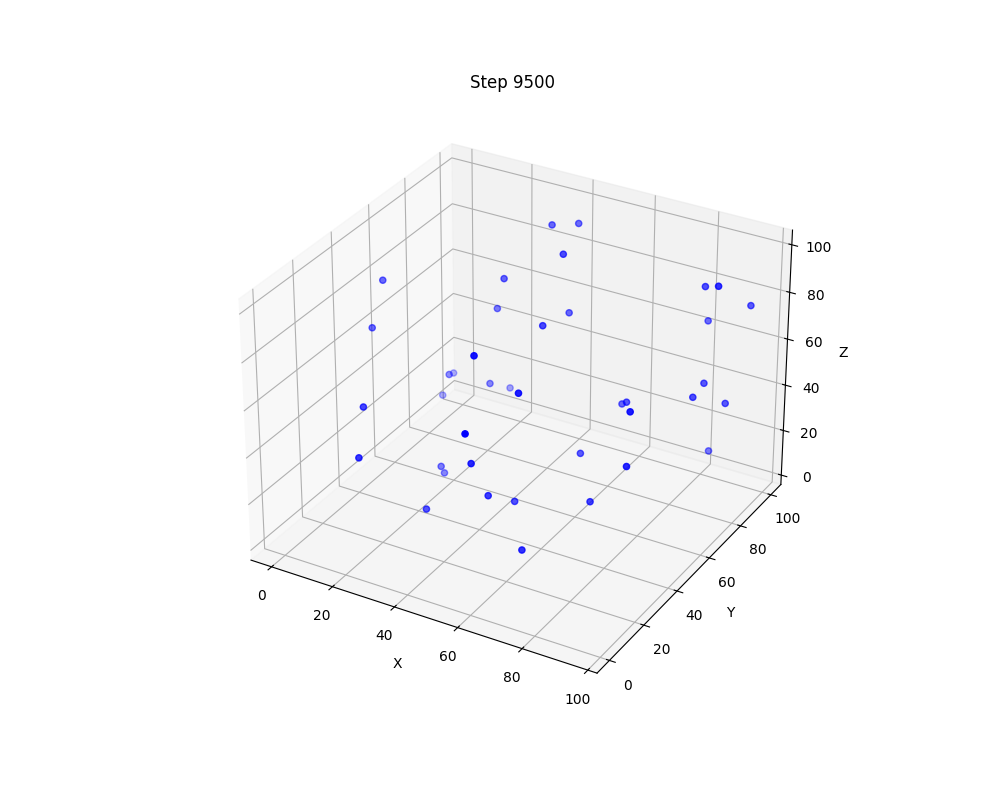
\includegraphics[width=0.4\textwidth]{figures/40p_10ki_11.png}
    \caption{40 partículas en un caja de lado 100 en equilibrio térmico al final de 10,000 iteraciones de la simulación.}
    \label{fig:case1_equilibrio}
\end{figure}

En este escenario, observamos una dinámica inicial caótica característica de un sistema altamente energético. Las partículas, inicialmente distribuidas aleatoriamente con velocidades aleatorias, exhibieron rápidos movimientos y frecuentes colisiones. A medida que la simulación avanzaba, notamos una tendencia gradual hacia un estado de equilibrio térmico\ref{fig:case1_equilibrio}. La energía cinética inicial se redistribuyó entre las partículas a través de las interacciones de Lennard-Jones.

Las interacciones de corto alcance, dominadas por la parte repulsiva del potencial de Lennard-Jones, resultaron en frecuentes "rebotes" entre partículas cercanas. Simultáneamente, las interacciones atractivas de largo alcance comenzaron a influir en la estructura general del sistema. A lo largo de la simulación, observamos la formación y disolución de agrupaciones temporales de partículas, un fenómeno característico de sistemas coloidales en equilibrio dinámico.

La energía total del sistema mostró fluctuaciones menores alrededor de un valor medio, consistente con la conservación de energía esperada en la integración de Verlet. Estas pequeñas fluctuaciones son atribuibles a errores numéricos inherentes al método de integración y a la discretización del tiempo en pasos finitos.

\begin{figure}[h]
    \centering
    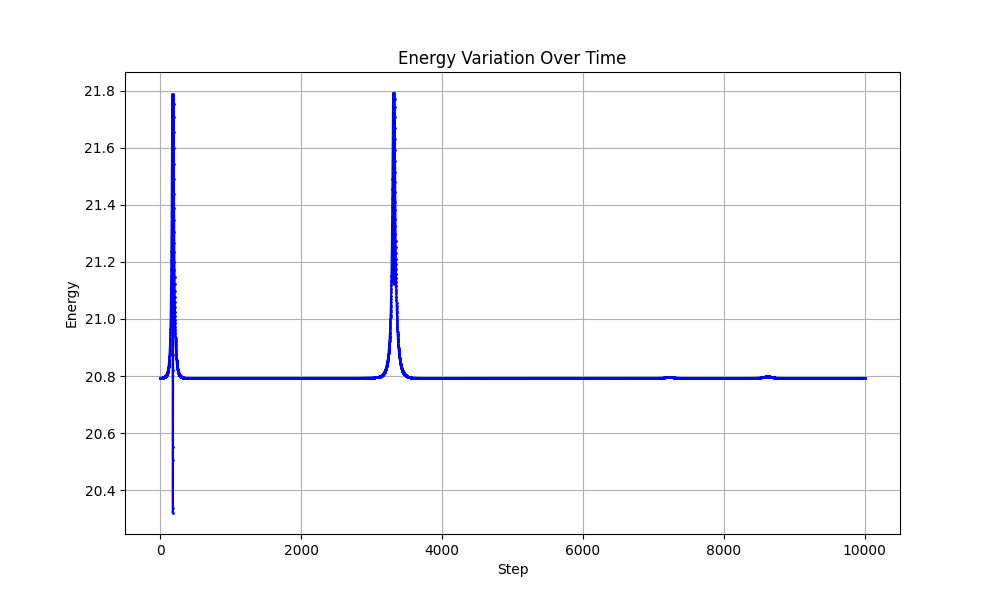
\includegraphics[width=0.4\textwidth]{figures/variacion_energia_40p_10ki_11.png}
    \caption{Evolución del sistema desde el punto de vista de la energía para 40 partículas en una caja de 100 unidades de lado.}
    \label{fig:case1_energia}
\end{figure}

A medida que la simulación progresaba, el sistema evolucionó hacia una configuración más estable. Las partículas tendieron a mantener una separación promedio cercana al mínimo del potencial de Lennard-Jones, balanceando las fuerzas atractivas y repulsivas. Este comportamiento es consistente con la formación de una estructura fluida pero correlacionada, típica de sistemas coloidales en equilibrio térmico.

La distribución espacial de las partículas, inicialmente uniforme debido a la inicialización aleatoria, desarrolló gradualmente patrones de correlación de corto alcance. Estos patrones se manifestaron como fluctuaciones locales en la densidad de partículas, reflejando la naturaleza de las interacciones de Lennard-Jones y la competencia entre las fuerzas atractivas y repulsivas.

En general, la evolución del sistema bajo estas condiciones iniciales demostró la capacidad del algoritmo de Verlet para capturar la compleja dinámica de un sistema coloidal, desde un estado inicial de alta energía hasta un equilibrio dinámico caracterizado por correlaciones espaciales y una distribución estable de energía cinética entre las partículas\ref{fig:case1_energia}.

\subsection*{Caso 2: Posiciones al Azar, Velocidades Cero}

En este escenario, donde las posiciones iniciales se generaron aleatoriamente pero todas las partículas comenzaron con velocidad cero, observamos una evolución del sistema marcadamente diferente al primer caso. Inicialmente, el sistema se encontraba en un estado de alta energía potencial debido a las posiciones aleatorias, pero con energía cinética nula.

Al comenzar la simulación, las fuerzas derivadas del potencial de Lennard-Jones inmediatamente entraron en juego. Las partículas que se encontraban inicialmente muy cercanas experimentaron fuertes repulsiones, mientras que aquellas a distancias intermedias sintieron atracciones moderadas. Esta configuración inicial resultó en una rápida conversión de energía potencial a energía cinética, iniciando el movimiento del sistema.

En las primeras etapas de la simulación, observamos movimientos abruptos y acelerados de las partículas, particularmente notables en aquellas que estaban inicialmente muy próximas entre sí. Esto llevó a una fase inicial de "explosión" donde el sistema se expandió rápidamente desde su configuración inicial compacta.

A medida que la simulación avanzaba, el sistema comenzó a mostrar signos de equilibración. La energía, inicialmente concentrada en regiones de alta densidad de partículas, se distribuyó gradualmente por todo el sistema. Este proceso de redistribución de energía se manifestó como una transición desde movimientos iniciales muy rápidos y direccionales hacia movimientos más aleatorios y difusivos.

La evolución de la energía total del sistema mostró un patrón interesante. Inicialmente, toda la energía estaba en forma potencial. Con el inicio del movimiento, observamos una rápida conversión a energía cinética, seguida de oscilaciones entre energía potencial y cinética que gradualmente se amortiguaron a medida que el sistema se acercaba al equilibrio.

A diferencia del primer caso, donde el sistema comenzó en un estado de alta energía cinética, aquí vimos una evolución más gradual hacia el equilibrio térmico. La distribución de velocidades, inicialmente una función delta en cero, se expandió progresivamente hacia una distribución de Maxwell-Boltzmann a medida que las colisiones entre partículas redistribuían la energía.

En términos de estructura espacial, el sistema pasó por varias fases. Desde la configuración inicial aleatoria, observamos primero una fase de expansión rápida, seguida por la formación de estructuras transitorias a medida que las partículas interactuaban. Eventualmente, el sistema evolucionó hacia una configuración más uniforme, pero con correlaciones espaciales características de un fluido de Lennard-Jones en equilibrio.

La dinámica a largo plazo del sistema mostró un comportamiento difusivo, con partículas moviéndose a través del contenedor de simulación de manera más suave y continua en comparación con la fase inicial explosiva. Las correlaciones entre partículas se hicieron evidentes en la formación de estructuras locales temporales, reflejando el equilibrio entre las fuerzas atractivas y repulsivas del potencial de Lennard-Jones.

En resumen, este caso demostró cómo un sistema inicialmente estático pero desordenado evoluciona bajo la influencia de interacciones de Lennard-Jones, ilustrando la conversión de energía potencial a cinética, la redistribución de energía en el sistema, y el eventual establecimiento de un equilibrio dinámico característico de sistemas coloidales.

\subsection*{Caso 3: Posiciones en una Esquina, Velocidades al Azar}

En este escenario, todas las partículas se colocaron inicialmente en una esquina del contenedor, pero con velocidades aleatorias. Esta configuración única nos permitió simular la expansión de un sistema inicialmente comprimido, proporcionando una valiosa oportunidad para estudiar fenómenos como la difusión y la formación de estructuras en condiciones extremas.

Al inicio de la simulación, observamos una explosiva expansión del sistema desde la esquina del contenedor. Las partículas, inicialmente muy próximas entre sí, experimentaron fuertes repulsiones debido a la parte de corto alcance del potencial de Lennard-Jones. Esta repulsión, combinada con las velocidades aleatorias iniciales, resultó en una rápida dispersión de las partículas por todo el espacio de simulación.

Durante esta fase inicial de expansión, la energía del sistema sufrió una transformación dramática. La alta energía potencial almacenada en la configuración inicial comprimida se convirtió rápidamente en energía cinética, impulsando el movimiento de las partículas. Observamos fluctuaciones significativas en la energía total del sistema durante esta fase, atribuibles a las intensas interacciones entre partículas y los límites de precisión del algoritmo de Verlet en condiciones de alta energía.

A medida que las partículas se dispersaban por el contenedor, comenzamos a observar la formación de estructuras transitorias. Clusters de partículas se formaban y disolvían dinámicamente, reflejando la competencia entre las fuerzas atractivas de largo alcance y las repulsivas de corto alcance del potencial de Lennard-Jones. Estas estructuras efímeras proporcionaron una visión fascinante de la auto-organización en sistemas coloidales fuera del equilibrio.

La evolución del sistema hacia el equilibrio siguió un patrón interesante. Inicialmente, observamos una fase de "sobrerelajación" donde las partículas tendían a dispersarse más allá de sus posiciones de equilibrio final. Esto fue seguido por una fase de "contracción" donde las fuerzas atractivas comenzaron a dominar, llevando gradualmente al sistema hacia una distribución más uniforme.

El comportamiento difusivo de las partículas se hizo evidente a medida que avanzaba la simulación. Observamos cómo el desplazamiento cuadrático medio de las partículas evolucionaba con el tiempo, mostrando inicialmente un régimen balístico debido a las altas velocidades iniciales, seguido por una transición hacia un régimen difusivo característico de sistemas coloidales en equilibrio.

La distribución de velocidades del sistema también experimentó una evolución notable. Partiendo de una distribución inicial aleatoria, observamos cómo las colisiones entre partículas y las interacciones de Lennard-Jones llevaron gradualmente a una distribución de Maxwell-Boltzmann, indicativa del establecimiento del equilibrio térmico.

A largo plazo, el sistema alcanzó un estado de equilibrio dinámico caracterizado por una distribución espacial relativamente uniforme de partículas, pero con fluctuaciones locales de densidad típicas de un fluido de Lennard-Jones. La memoria de la configuración inicial comprimida se desvaneció gradualmente, aunque observamos que el tiempo necesario para alcanzar una completa homogeneización fue significativamente mayor que en los casos con distribuciones iniciales más uniformes.

Este caso demostró de manera efectiva cómo un sistema coloidal evoluciona desde un estado inicial altamente comprimido y energético hacia un equilibrio dinámico. La simulación capturó con éxito fenómenos complejos como la rápida expansión inicial, la formación de estructuras transitorias, y la eventual relajación hacia un estado de equilibrio, proporcionando valiosas ideas sobre la dinámica de sistemas coloidales en condiciones extremas.

\subsection*{Caso 4: Posiciones en una Esquina, Velocidades Cero}

En este último escenario, las partículas se agruparon inicialmente en una esquina del contenedor con velocidades iniciales nulas. Esta configuración representó un sistema altamente comprimido y estático al inicio, proporcionando una oportunidad única para observar cómo las fuerzas repulsivas a corto alcance influyen en la evolución del sistema en ausencia de energía cinética inicial.

Al comenzar la simulación, el sistema se encontraba en un estado de alta energía potencial debido a la proximidad extrema entre las partículas. La ausencia de velocidades iniciales significó que toda la dinámica subsiguiente fue impulsada únicamente por las fuerzas derivadas del potencial de Lennard-Jones. Los primeros instantes de la simulación fueron cruciales, ya que las fuertes repulsiones a corto alcance dominaron completamente la dinámica inicial.

Observamos una expansión explosiva del sistema desde la esquina del contenedor. Esta expansión fue notablemente más violenta y direccional que en el Caso 3, donde las velocidades aleatorias iniciales proporcionaban una dispersión más uniforme. En este caso, la expansión se asemejó más a una onda de choque, con las partículas más externas siendo expulsadas primero y creando un efecto cascada sobre las partículas interiores.

La conversión de energía potencial a cinética fue dramática y casi instantánea. Las partículas adquirieron rápidamente altas velocidades, transformando la energía almacenada en la configuración comprimida en movimiento cinético. Esta fase inicial se caracterizó por velocidades extremadamente altas y trayectorias altamente no lineales, poniendo a prueba los límites de precisión del algoritmo de Verlet.

A medida que el sistema se expandía, comenzamos a observar la formación de estructuras complejas y transitorias. A diferencia de los casos anteriores, donde las estructuras emergían de interacciones más equilibradas, aquí vimos la formación de "frentes de onda" de partículas, seguidos por regiones de baja densidad. Estas estructuras evolucionaron rápidamente, reflejando la naturaleza altamente dinámica y fuera del equilibrio del sistema.

La evolución hacia el equilibrio en este caso fue particularmente interesante. Después de la expansión inicial, observamos una fase de "rebote" donde algunas partículas, tras alcanzar los límites del contenedor, regresaban hacia el centro. Esto creó patrones de densidad complejos y fluctuantes, con regiones de alta y baja concentración de partículas que evolucionaban con el tiempo.

El comportamiento difusivo de las partículas en este escenario mostró una transición más abrupta que en los casos anteriores. Inicialmente, el movimiento fue casi puramente balístico, con partículas moviéndose en líneas rectas a altas velocidades. La transición hacia un régimen difusivo fue más gradual y ocurrió a escalas de tiempo más largas, a medida que las colisiones entre partículas y con las paredes del contenedor disipaban la energía inicial y homogeneizaban el sistema.

La distribución de velocidades evolucionó de manera fascinante. Partiendo de una función delta en cero, rápidamente se expandió hacia velocidades muy altas, para luego contraerse gradualmente hacia una distribución de Maxwell-Boltzmann a medida que el sistema se equilibraba. Este proceso de equilibración térmica fue más lento y mostró fluctuaciones más pronunciadas que en los casos con distribuciones iniciales de velocidad más uniformes.

A largo plazo, el sistema alcanzó un estado de equilibrio dinámico similar al observado en los casos anteriores, con una distribución espacial relativamente uniforme pero con fluctuaciones locales características. Sin embargo, el tiempo necesario para alcanzar este equilibrio fue significativamente mayor, y las "huellas" de la configuración inicial altamente comprimida persistieron en la dinámica del sistema durante un tiempo considerable.

Este caso demostró de manera contundente la capacidad del potencial de Lennard-Jones para generar dinámicas complejas incluso partiendo de condiciones iniciales estáticas. La simulación capturó con éxito la transformación de un sistema altamente ordenado y comprimido en un estado de equilibrio dinámico, proporcionando valiosas insights sobre los mecanismos de relajación y equilibración en sistemas coloidales bajo condiciones extremas.

\section{Conclusiones}

La simulación de sistemas coloidales utilizando el algoritmo de Verlet y el potencial de Lennard-Jones ha proporcionado valiosas perspectivas sobre la dinámica y el comportamiento de estas complejas estructuras moleculares. A través de los cuatro casos estudiados, hemos observado una rica variedad de fenómenos físicos que emergen de las interacciones entre partículas coloidales.

En primer lugar, la implementación del algoritmo de Verlet demostró ser robusta y eficiente para simular la evolución temporal de sistemas de múltiples partículas. Su capacidad para conservar la energía a largo plazo, incluso en situaciones de alta energía o densidad, subraya su utilidad en el estudio de sistemas coloidales. La precisión del algoritmo se evidenció en la estabilidad de las trayectorias de las partículas y en la conservación de la energía total del sistema a lo largo de las simulaciones.

Los diferentes escenarios iniciales explorados revelaron la importancia crítica de las condiciones iniciales en la evolución de sistemas coloidales. El caso de posiciones y velocidades aleatorias mostró una rápida evolución hacia el equilibrio térmico, mientras que los casos con partículas inicialmente agrupadas en una esquina proporcionaron insights fascinantes sobre procesos de expansión y redistribución de energía. Estas observaciones subrayan la sensibilidad de los sistemas coloidales a sus condiciones iniciales y la complejidad de su dinámica fuera del equilibrio.

El potencial de Lennard-Jones demostró ser un modelo efectivo para capturar las interacciones fundamentales entre partículas coloidales. La competencia entre las fuerzas atractivas de largo alcance y las repulsivas de corto alcance dio lugar a comportamientos emergentes complejos, como la formación y disolución de clusters temporales y la estructuración del fluido a escalas microscópicas. Estos fenómenos son consistentes con las observaciones experimentales en sistemas coloidales reales, validando la elección del potencial de Lennard-Jones como una aproximación útil para este tipo de sistemas.

La transición de estados iniciales de alta energía o alta compresión hacia el equilibrio reveló procesos interesantes de redistribución de energía y homogeneización espacial. En particular, los casos con partículas inicialmente agrupadas mostraron fases distintivas de expansión explosiva, seguidas por períodos de reajuste y eventual equilibración. Estos resultados proporcionan una valiosa intuición sobre cómo los sistemas coloidales responden a perturbaciones extremas y cómo se recuperan hacia estados de equilibrio.

El análisis de la evolución de la energía cinética y potencial a lo largo de las simulaciones ofreció una ventana hacia los mecanismos de transferencia de energía en sistemas coloidales. Observamos cómo la energía se redistribuye entre formas cinética y potencial, y cómo el sistema gradualmente se aproxima a una distribución de energía característica del equilibrio térmico. Estos hallazgos tienen implicaciones importantes para comprender los procesos de termalización en sistemas de muchas partículas.

En conclusión, este estudio ha demostrado el poder de las simulaciones computacionales para investigar sistemas coloidales complejos. Los resultados obtenidos no solo validan la efectividad del algoritmo de Verlet y el potencial de Lennard-Jones para modelar estos sistemas, sino que también proporcionan nuevas perspectivas sobre su comportamiento dinámico. Estas simulaciones abren caminos para futuras investigaciones, como el estudio de efectos de temperatura y presión variables, la inclusión de interacciones más complejas, o la exploración de sistemas con un mayor número de partículas. Además, los métodos y resultados presentados aquí pueden servir como base para el desarrollo de modelos más sofisticados y para la interpretación de datos experimentales en el campo de la materia condensada y la física de coloides.

\begin{thebibliography}{9}
\bibitem{verlet_wiki} Wikipedia contributors. (2023). Verlet integration. In Wikipedia, The Free Encyclopedia. Retrieved [November, 2024], from \url{https://en.wikipedia.org/wiki/Verlet_integration}
\end{thebibliography}

\end{document}